\documentclass[conference]{IEEEtran}
\IEEEoverridecommandlockouts
% The preceding line is only needed to identify funding in the first footnote. If that is unneeded, please comment it out.
%Template version as of 6/27/2024

\usepackage{cite}
\usepackage{amsmath,amssymb,amsfonts}
\usepackage{algorithmic}
\usepackage{graphicx}
\usepackage{textcomp}
\usepackage{xcolor}
\def\BibTeX{{\rm B\kern-.05em{\sc i\kern-.025em b}\kern-.08em
    T\kern-.1667em\lower.7ex\hbox{E}\kern-.125emX}}
\begin{document}

\title{CLARITY - UNMASKING POLITICAL QUESTION EVASIONS}

\author{\IEEEauthorblockN{Taha Munawar}
\IEEEauthorblockA{\textit{Department of Computer Science} \\
\textit{Habib University}\\
Karachi, Pakistan \\
tm08122@st.habib.edu.pk}
\and
\IEEEauthorblockN{Basil Ali Khan}
\IEEEauthorblockA{\textit{Department of Computer Science} \\
\textit{Habib University}\\
Karachi, Pakistan \\
bk08221@st.habib.edu.pk}
\and
\IEEEauthorblockN{Arsal Jangda}
\IEEEauthorblockA{\textit{Department of Computer Science} \\
\textit{Habib University}\\
Karachi, Pakistan \\
aj08514@st.habib.edu.pk}
\and
\IEEEauthorblockN{Sarfaraz Baig}
\IEEEauthorblockA{\textit{Department of Computer Science} \\
\textit{Habib University}\\
Karachi, Pakistan \\
sb08112@st.habib.edu.pk}
\and
\IEEEauthorblockN{Sandesh Kumar}
\IEEEauthorblockA{\textit{Department of Computer Science} \\
\textit{Habib University}\\
Karachi, Pakistan \\
sandesh.kumar@sse.habib.edu.pk}
\and
\IEEEauthorblockN{Abdul Samad}
\IEEEauthorblockA{\textit{Department of Computer Science} \\
\textit{Habib University}\\
Karachi, Pakistan \\
abdul.samad@sse.habib.edu.pk}
}

\maketitle

\begin{abstract}
This paper details our submission for SemEval Task 6: CLARITY - Unmasking Political Question Evasions. The task focuses on categorizing question-answer pairs from political interviews using a two-level hierarchical taxonomy. The objective is to classify each response by both its high-level ``clarity'' and its specific fine-grained ``evasion technique''. This work aims to advance the automated detection of political equivocation. We present novel methodologies designed to build upon the baseline models from \cite{b4} and improve classification performance on this task.
\end{abstract}

\begin{IEEEkeywords}
evasion detection, political discourse, text classification, political equivocation.
\end{IEEEkeywords}

\section{Introduction}
In high-stakes public discourse, particularly in political interviews, the clarity of a response is often as important as its content. The phenomenon of ``equivocation'' or ``evasion'' (the act of responding to a question without directly answering it) is a well-documented strategy used to navigate difficult topics, deflect scrutiny, or manage public perception. While this has been extensively studied in political science and linguistics, the automated detection and classification of such ambiguous responses present a complex challenge for Natural Language Processing (NLP).

This challenge was formally framed as a discrete NLP task by Thomas et al. \cite{b4} in their paper: ``I Never Said That'': A dataset, taxonomy and baselines on response clarity classification.

The central research question defined by \cite{b4} is: \textbf{How can we automatically and systematically evaluate the clarity of a given response with respect to its corresponding question?}

To address this, a novel two-level hierarchical taxonomy was developed to capture the nuances of response clarity, as shown in Fig \ref{fig:taxonomy}. The first level, Clarity, provides a high-level evaluation of the response's overall directness and completeness in relation to the question. The second level, Evasion, identifies the specific fine-grained linguistic technique or strategy used by the speaker.

Subtask1 and Subtask 2 of SemEval Task 6 focus on predicting the Clarity and Evasion levels, respectively, for given question-answer pairs from political interviews.

The explanation of the taxonomy label for each level is as follows:

\textbf{Clarity Level Categories:}

\begin{itemize}
    \item \textbf{Clear Reply:} Information is explicitly provided.
    \item \textbf{Clear Non-Reply:} Information is openly refused.
    \item \textbf{Ambivalent Reply:} The response is related but evasive.
\end{itemize}

\textbf{Evasion Level Categories:}

\begin{itemize}
    \item \textbf{Explicit:} The information requested is explicitly stated (in the requested form).
    \item \textbf{Implicit:} The information requested is given, but without being explicitly stated (not in the expected form).
    \item \textbf{General:} The information provided is too general or lacks the requested specificity.
    \item \textbf{Partial:} Offers only a specific component of the requested information.
    \item \textbf{Dodging:} Ignores the question altogether.
    \item \textbf{Deflection:} Starts on topic but shifts the focus and makes a different point than what is asked.
    \item \textbf{Declining to answer:} Acknowledges the question but directly or indirectly refuses to answer at the moment.
    \item \textbf{Claims ignorance:} The answerer claims or admits not to know the answer themselves.
    \item \textbf{Clarification:} Does not provide the requested information and instead asks for clarification.
\end{itemize}

\begin{figure}[h!]
    \centering
    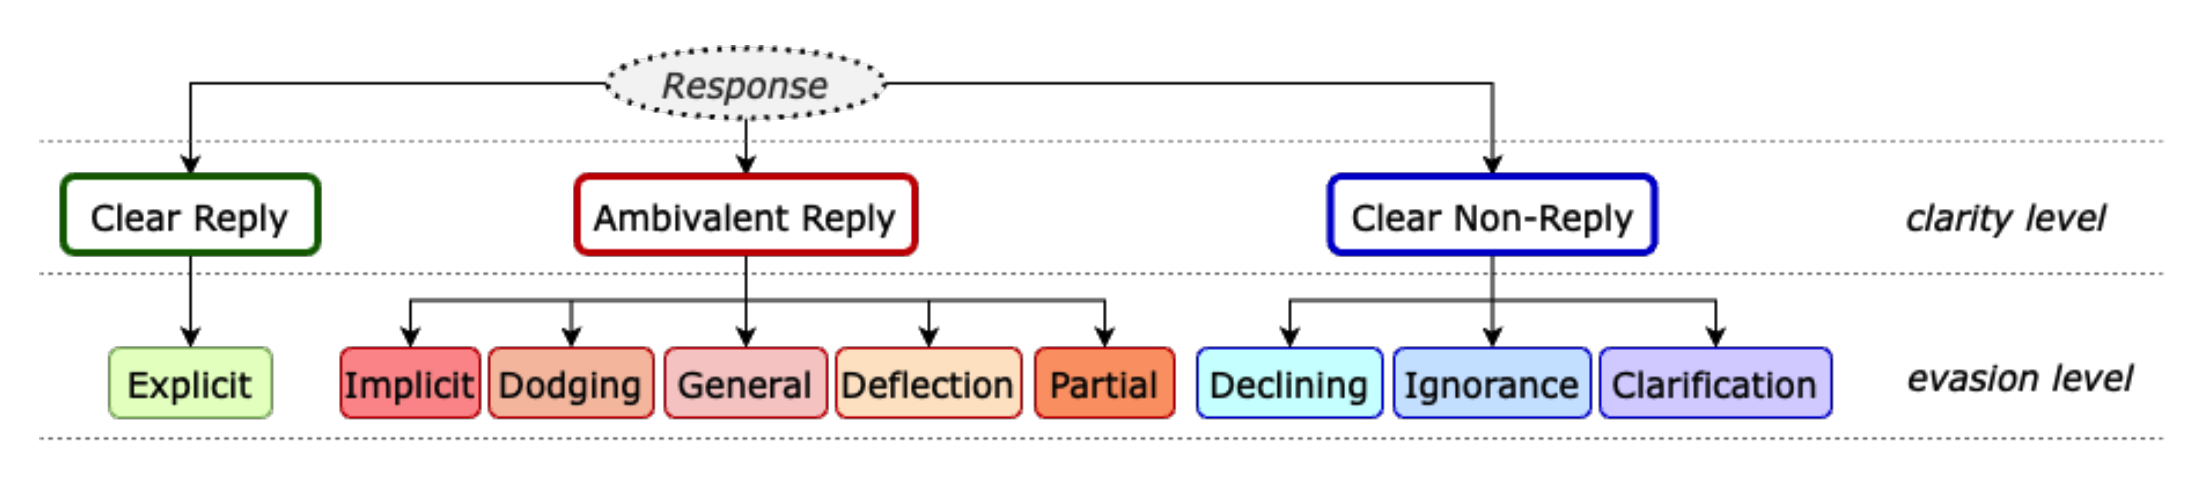
\includegraphics[width=0.9\linewidth]{taxonomy.png}
    \caption{Two-level hierarchical taxonomy for evaluating response clarity.}
    \label{fig:taxonomy}
\end{figure}

\section{Dataset}

The data was sourced from 287 unique interview transcripts of US presidents from 2006 to 2023. The transcripts were taken directly from the official White House website.

A significant challenge identified by the authors was the prevalence of ``multi-barrelled'' questions, where interviewers pose multiple, distinct questions within a single turn. They noted that this complicates the annotation, as a politician might clearly answer one part of the question while evading another.

To address this, they adopted a fine-grained decomposition strategy. First, ChatGPT was leveraged to parse the transcripts and break down these complex, multi-part questions into their constituent ``singular QA pairs'' (sQAs). Each sQA pair consists of a single subquestion from the multi-barrelled question and the complete response from the politician, to determine how that particular question was answered in the context of the full response. An example of this decomposition is shown below:

\begin{quote}
\small % Makes the example text slightly smaller
\textbf{Original Multi-barrelled Question:} \\
\textit{Q. Is there a reason your press staff was unaware of that? And what did you say to the Chinese President?}

\smallskip % Adds a small vertical space
\textbf{Original Full Answer:} \\
\textit{Well—and they weren't with me the entire time. Look, I made it clear that I thought that China had an obligation to be more forthcoming on exactly what the source of the virus was and where it came from.Yes.}

\smallskip

\textbf{Resulting sQA Pair 1:}
\begin{itemize}
    \item \textbf{Sub-question:} \textit{Is there a reason your press staff was unaware of that?}
    \item \textbf{Full Answer:} \textit{Well—and they weren't with me the entire time. Look, I made it clear that I thought that China had an obligation to be more forthcoming on exactly what the source of the virus was and where it came from.Yes.}
\end{itemize}

\textbf{Resulting sQA Pair 2:}
\begin{itemize}
    \item \textbf{Sub-question:} \textit{What did you say to the Chinese President?}
    \item \textbf{Full Answer:} \textit{Well—and they weren't with me the entire time. Look, I made it clear that I thought that China had an obligation to be more forthcoming on exactly what the source of the virus was and where it came from.Yes.}
\end{itemize}
\end{quote}

The resulting dataset had two splits: a training set with 3,450 rows and a test set with 308 rows, with the important columns being ``interview\_question'', ``interview\_answer'', ``question'' ``clarity\_label'', and ``evasion\_label''.

We noted that the evasion\_label column was empty in the test set. The researchers clarified this was intentional. They found that annotators had disagreements (high variance) when assigning these labels, so they decided against using a single ``ground truth'' label.

Instead, the test set provides the individual labels from three annotators in the ``annotator1'', ``annotator2'', and ``annotator3'' columns. For evasion level prediction, a model's prediction is considered correct if it matches any of these three labels.

Moreover, the dataset exhibited significant class imbalance in both clarity and evasion labels, as shown in the figures below.

\begin{figure}[h!]
    \centering
    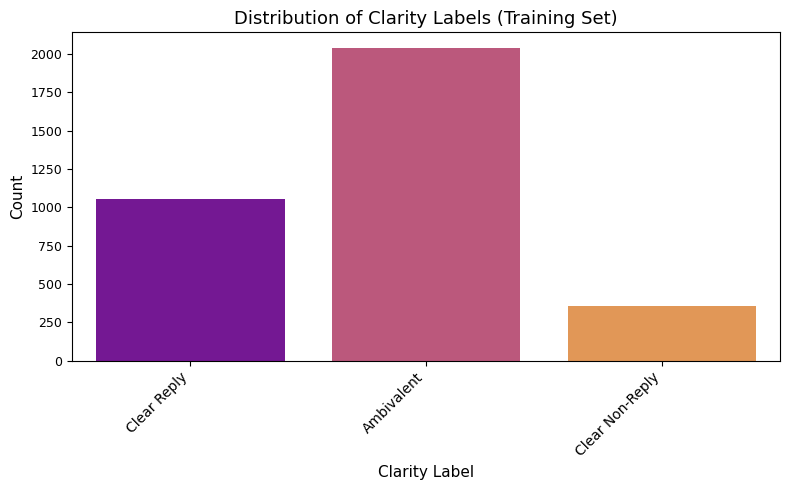
\includegraphics[width=0.9\linewidth]{clarity_count.png}
    \caption{Distribution of clarity level labels in the dataset.}
    \label{fig:clarity_count}
\end{figure}

\begin{figure}[h!]
    \centering
    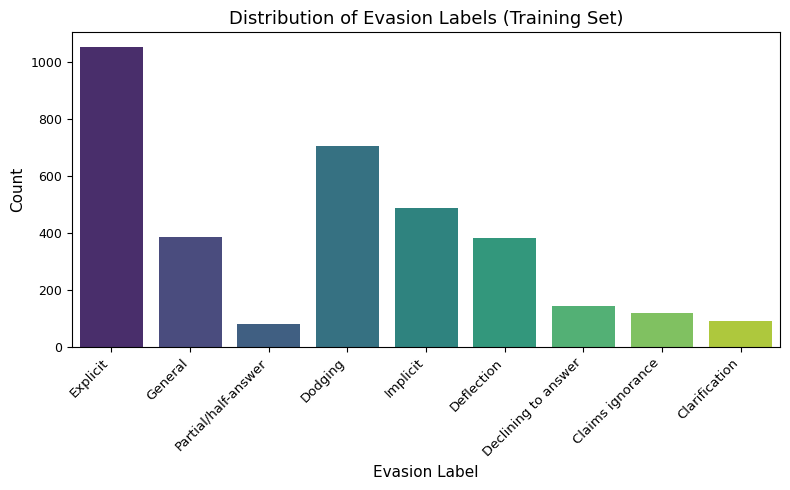
\includegraphics[width=0.9\linewidth]{evasion_count.png}
    \caption{Distribution of evasion level labels in the dataset.}
    \label{fig:evasion_count}
\end{figure}

\section{Literature Review}

The automatic detection of political question evasion draws on research in ambiguity detection and political text analysis. This section reviews key studies that inform our approach.

Shi et al. \cite{b1} tackle the challenge of identifying ambiguous questions in large language model (LLM) question-answering systems. They show that LLMs can generate coherent responses but often fail to recognize questions with multiple interpretations, a common strategy in political discourse. Their method combines LLM-generated multiple answers (via self-consistency prompting) with a lightweight Random Forest classifier that measures answer variance to predict ambiguity. This approach outperforms prompt-based and larger transformer baselines, especially with limited labeled data. For our work, their technique is relevant because political evasion often appears as subtle ambiguity in answers, and their low-resource success mirrors real-world constraints in political datasets.

Liu et al. \cite{b2} examine how well language models handle ambiguity through the AMBIENT benchmark, a linguist-annotated dataset of lexical, syntactic, and pragmatic ambiguities, including political claims. They find that even advanced models like GPT-4 struggle to disambiguate meanings as effectively as humans. However, fine-tuned multilabel NLI models can flag ambiguous or misleading claims “in the wild.” This insight is crucial for our project: political evasion frequently relies on ambiguity, and the limits of current models highlight the need for domain-specific detection methods.

Chatsiou and Mikhaylov \cite{b3} survey the use of deep learning in political text analysis, tracing the shift from feature-engineered models to contextual transformers such as BERT. They show that deep models capture nuance and context, essential for interpreting political communication, where subtext and intent are key. Their discussion of transfer learning, annotation efficiency, and ethical issues underscores the importance of scalable and transparent systems for tasks like evasion detection.

While the previously mentioned studies focus on computational ambiguity detection, a separate body of work in linguistics and political science provides the theoretical foundation for evasion taxonomies, like the one used in this SemEval task. These studies deconstruct the act of ``not answering'' into a set of discrete, observable rhetorical strategies.

For example, Gabrielsen et al \cite{b5} define ``shifting'' as a subtle evasion where the interviewee seemingly accepts the question but ``refocuses'' the question replacing its critical aspect with a more favorable one, a direct analogue to the ``Deflection'' label. They, along with Mahdi \& Al-Azzawi \cite{b6}, identify common patterns like shifts in time, agent, or abstraction level, as well as ``Redirection'' and ``Non-answers''.

Mahdi \& Al-Azzawi \cite{b6} provide the formal pragmatic theory that unites these observations: evasion functions by flouting Grice's Maxims. This framework provides a mechanism for understanding the SemEval taxonomy: \begin{itemize} \item A response labeled ``Dodging'' or ``Deflection'' is fundamentally flouting the Maxim of Relation (relevance). \item A response labeled ``General'' or ``Partial'' is flouting the Maxim of Quantity (informativeness). \end{itemize}

Other studies provide granular, linguistic-level examples that somewhat map to our labels. Vázquez Carranza's \cite{b7} ``non-type-conforming answers'' (e.g., giving a general description instead of a specific number)  aligns  with the ``General'' label. Similarly, Abidin et al. identify ``minimizing the divergence'' (e.g., calling an incident an ``isolated case''), which fits the ``Partial'' or ``General'' labels. These works also categorize confrontational tactics like ``attacking the questioner'' or ``challenging professionalism'', which are forms of ``Dodging'' or ``Deflection''.

While these papers do not propose computational models, nor do they provide annotated datasets which we can utilize for model training, they offer a theoretical underpinning for the taxonomy used in this SemEval task. Perhaps we can leverage some of their linguistic insights to engineer features or augment our training data. More importantly, they validate the taxonomy's relevance and comprehensiveness for capturing the multifaceted nature of political evasion.

A key computational limitation, noted by the task organizers in \cite{b8}, is that traditional classifiers like BERT are limited to 512 tokens, forcing the truncation of long sQA pairs. This truncation risks cutting off the very part of the answer that contains the evasion. The recent introduction of ModernBERT  directly addresses this. This modernized encoder features a native 8192 sequence length. This expanded context window is highly relevant to our work, as it allows our model to process the entire sQA to capture the full context of a long, complex answer.

Lastly, Alvarez \& Morrier \cite{b9} offer a valuable domain pre-adaptation strategy using their large dataset of 58,343 Canadian Question Period exchanges. They trained a Sentence-BERT model to measure answer ``quality'' via cosine similarity between question-answer embeddings, learned self-supervisedly by identifying correct answers from negative samples .

This is highly relevant because we can pre-train our classifier (like ModernBERT) on their political Q\&A dataset using this same cosine similarity objective. This allows the model to learn the specific discourse patterns of political Q\&As before fine-tuning on the SemEval evasion task, potentially improving performance.

\begin{thebibliography}{00}
\bibitem{b4} K. Thomas, G. Filandrianos, M. Lymperaiou, C. Zerva, and G. Stamou, ``I never said that: A dataset, taxonomy and baselines on response clarity classification,'' 2024, arXiv:2409.13879. [Online]. Available: https://arxiv.org/abs/2409.13879
\bibitem{b1} Z. Shi et al., ``Ambiguity detection and uncertainty calibration for question answering with large language models,'' in \textit{Proc. 5th Workshop on Trustworthy NLP (TrustNLP)}, 2025, pp. 41--55, doi: 10.18653/v1/2025.trustnlp-main.4.
\bibitem{b2} A. Liu et al., ``We're afraid language models aren't modeling ambiguity,'' in \textit{Proc. 2023 Conf. Empirical Methods in Natural Language Processing}, 2023, pp. 790--807, doi: 10.18653/v1/2023.emnlp-main.51.
\bibitem{b3} K. Chatsiou and S. J. Mikhaylov, \textit{Deep Learning for Political Science}. London, UK: SAGE Publications Ltd, 2020.
\bibitem{b5} J. Gabrielsen, H. Jønch-Clausen, and C. Pontoppidan, “Answering without answering: Shifting as an evasive rhetorical strategy,” Journalism, vol. 21, no. 9, pp. 1355–1370, Sep. 2020, doi: 10.1177/1464884917738412.
\bibitem{b6} S. H. Mahdi and Prof. Q. O. Al-Azzawi, “The Pragmatics of Dialogue Evasion in American Political Debates,” JPPS, no. 43, pp. 1–13, Apr. 2024, doi: 10.55529/jpps.43.1.13.
\bibitem{b7} A. Vázquez Carranza, “Evading and resisting answering: An analysis of Mexican Spanish news interviews,” PS, vol. 7, no. 4, pp. 570–594, Dec. 2016, doi: 10.1075/ps.7.4.03car.
\bibitem{b8} B. Warner et al., “Smarter, Better, Faster, Longer: A Modern Bidirectional Encoder for Fast, Memory Efficient, and Long Context Finetuning and Inference,” 2024, arXiv. doi: 10.48550/ARXIV.2412.13663.
\bibitem{b9} R. M. Alvarez and J. Morrier, “Measuring the Quality of Answers in Political Q\&As with Large Language Models,” Polit. Anal., pp. 1–18, Jul. 2025, doi: 10.1017/pan.2025.10007.
\end{thebibliography}

\end{document}
